\subsection*{Problema 14}
\textbf{Enunciado:} Evaluar la integral definida 
mediante sumas de Riemann:
\begin{align*}
\int_{0}^{1} (1 - x^3) \, dx
\end{align*}

\textbf{Solución:} 
Utilizamos la definición de la integral definida 
como el límite de una suma de Riemann por la 
derecha. Dividimos el intervalo $[0, 1]$ en $n$ 
subintervalos de ancho igual a:
\begin{align*}
\Delta x = \dfrac{1 - 0}{n} = \dfrac{1}{n}
\end{align*}

Los puntos de muestreo son $x_i = i \Delta x = \dfrac{i}{n}$ 
para $i = 1, 2, \dots, n$. Evaluamos la función 
$f(x) = 1 - x^3$ en estos puntos:
\begin{align*}
f(x_i) = 1 - \left(\dfrac{i}{n}\right)^3 = 1 - \dfrac{i^3}{n^3}
\end{align*}

Planteamos la suma de Riemann:
\begin{align*}
S_n &= \sum_{i=1}^{n} f(x_i) \Delta x \\
S_n &= \sum_{i=1}^{n} \left(1 - \dfrac{i^3}{n^3}\right) \dfrac{1}{n}
\end{align*}

Distribuimos el término $\dfrac{1}{n}$ y 
separamos la sumatoria:
\begin{align*}
S_n &= \dfrac{1}{n} \sum_{i=1}^{n} 1 
- \dfrac{1}{n^4} \sum_{i=1}^{n} i^3
\end{align*}

Aplicamos las fórmulas de suma conocidas 
$\sum_{i=1}^{n} 1 = n$ y 
$\sum_{i=1}^{n} i^3 = \left[\dfrac{n(n+1)}{2}\right]^2$:
\begin{align*}
S_n &= \dfrac{1}{n} (n) 
- \dfrac{1}{n^4} \left[\dfrac{n(n+1)}{2}\right]^2 \\
S_n &= 1 - \dfrac{n^2(n+1)^2}{4n^4}
\end{align*}

Simplificamos la expresión algebraica:
\begin{align*}
S_n &= 1 - \dfrac{1}{4} \left(\dfrac{n+1}{n}\right)^2 \\
S_n &= 1 - \dfrac{1}{4} \left(1 + \dfrac{1}{n}\right)^2
\end{align*}

Calculamos el límite cuando $n \to \infty$ 
para obtener el valor exacto de la integral:
\begin{align*}
\int_{0}^{1} (1 - x^3) \, dx &= \lim_{n \to \infty} S_n \\
&= \lim_{n \to \infty} \left[ 1 - \dfrac{1}{4} \left(1 + \dfrac{1}{n}\right)^2 \right] \\
&= 1 - \dfrac{1}{4} (1 + 0)^2 \\
&= 1 - \dfrac{1}{4} = \dfrac{3}{4}
\end{align*}

El valor de la integral definida es $\dfrac{3}{4}$.

\begin{figure}[H]
	\centering
	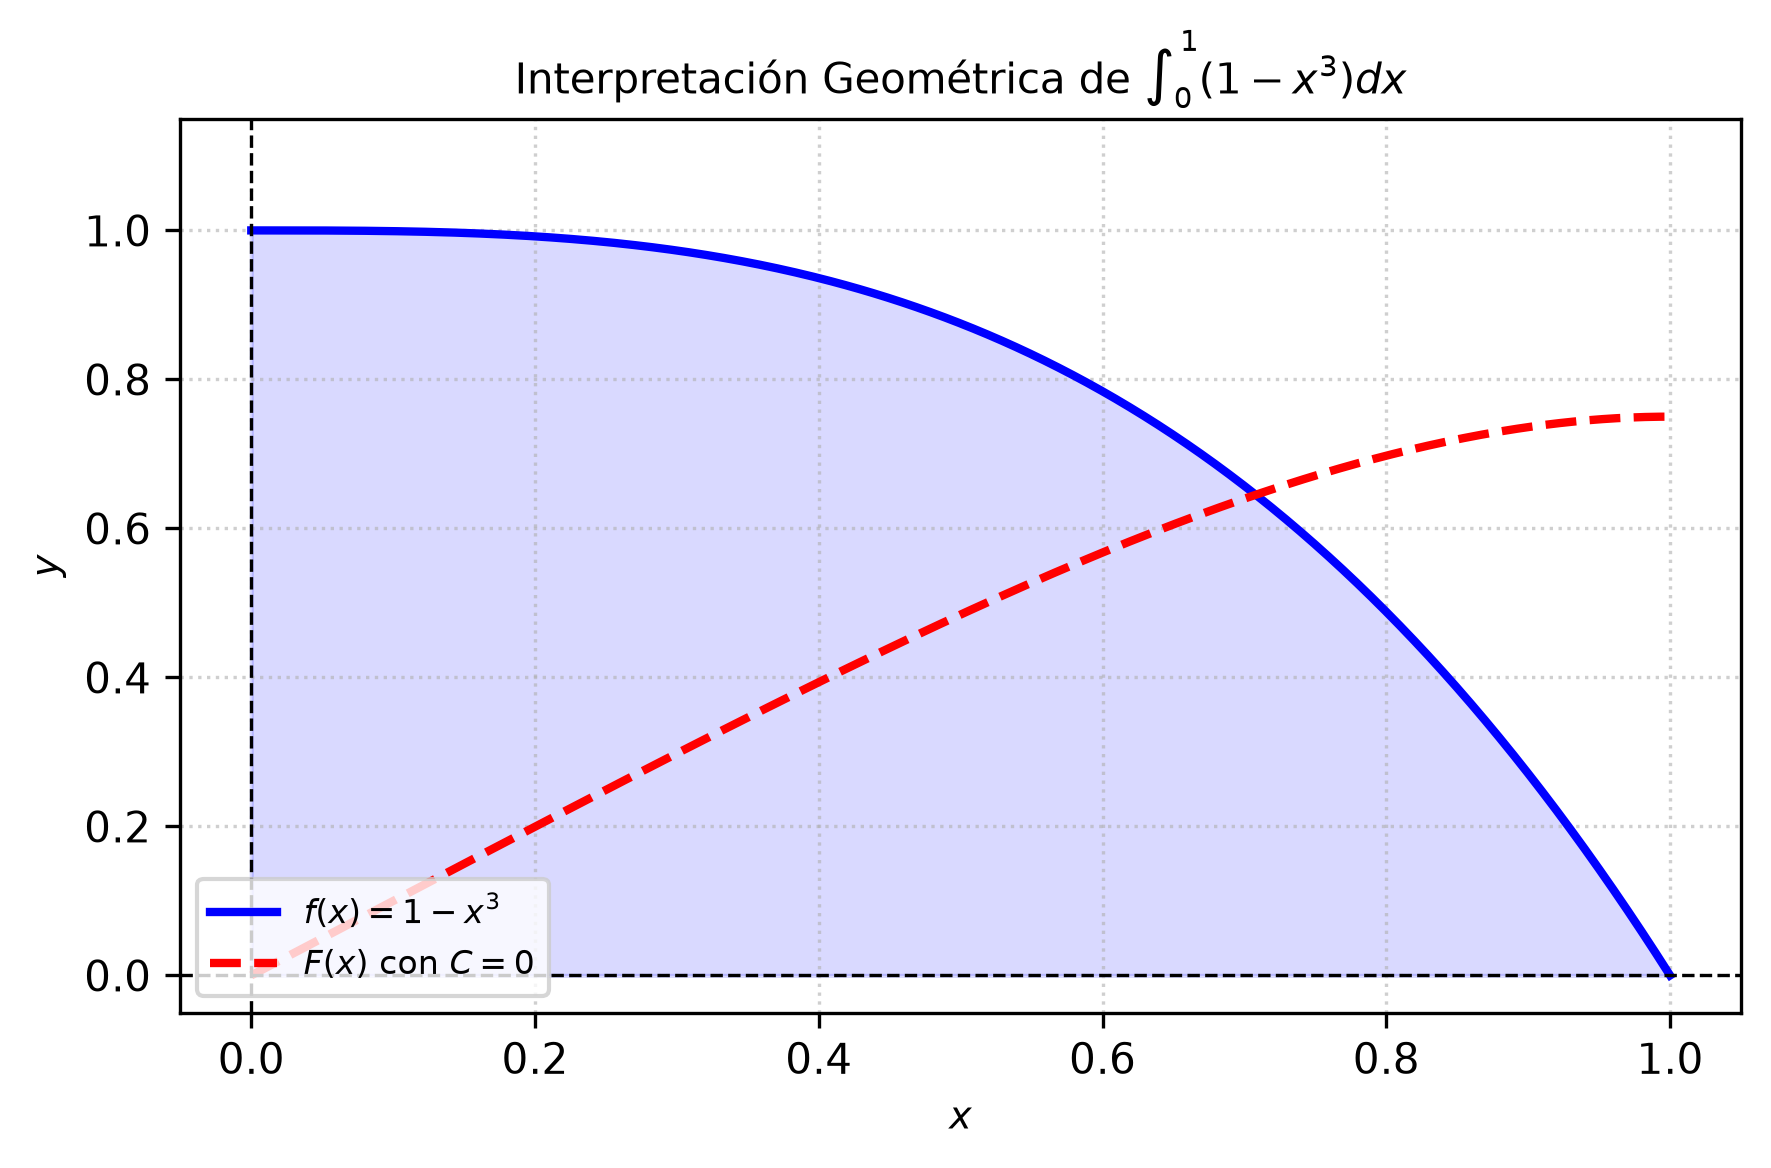
\includegraphics[width=\columnwidth]{semana_06/graficas/SEM06_P14_grafica.png}
	\caption{Representación gráfica de $f(x)$ y su antiderivada $F(x)$ evaluada para la constante de integración $C = 0$ (Problema 14).}
	\label{fig:problema14}
\end{figure}
